\section{Detailed isolation studies}
\label{app:iso}
Since one of the dominant background sources in the analysis is due to events with a non-prompt lepton, 
dedicated lepton isolation optimization studies have been performed.

For the DC14 walkthroughs in April 2015~\cite{NoteDC14}, the following cuts on the isolation variables were found 
to be optimal:
\begin{itemize}
\item Electrons: {\tt TightLLH}, ptvarcone20/\pt$<$0.06 and topoetcone20/\pt$<$0.06 (``FixedCutTight'')
\item Muons: ptvarcone30/\pt\ $<0.06$ (``FixedCutTightTrackOnly'')
\end{itemize}

Shortly after, the ATLAS isolation forum released pre-pre-recommendations for DC14 samples relying on the 
{\tt ElectronIsolationSelectionTool}~\cite{ElectronIso_twiki}. This tool parametrizes the cuts on the isolation variables 
as a function of the efficiency in $Z\to\ell\ell$ events.
The pre-pre-recommendations included working points with constant ({\tt Tight}, {\tt Medium}, {\tt Loose}, 
{\tt VeryLoose} and {\tt VeryLooseTrackOnly}) or with a variable efficiency as a function of $\pt$ ({\tt Gradient} and {\tt GradientLoose});
they relied on the relative isolation variables topoetcone20/\pt and ptvarcone20/\pt 
for electrons, and topoetcone20/\pt and ptvarcone30/\pt for muons. 
Optimization studies considering both signal and background using the discovery significance as figure of merit showed that the {\tt GradientLoose} working point had a good performance for the signal regions in this analysis.


%\begin{figure}[phtb!]
%\begin{center}
%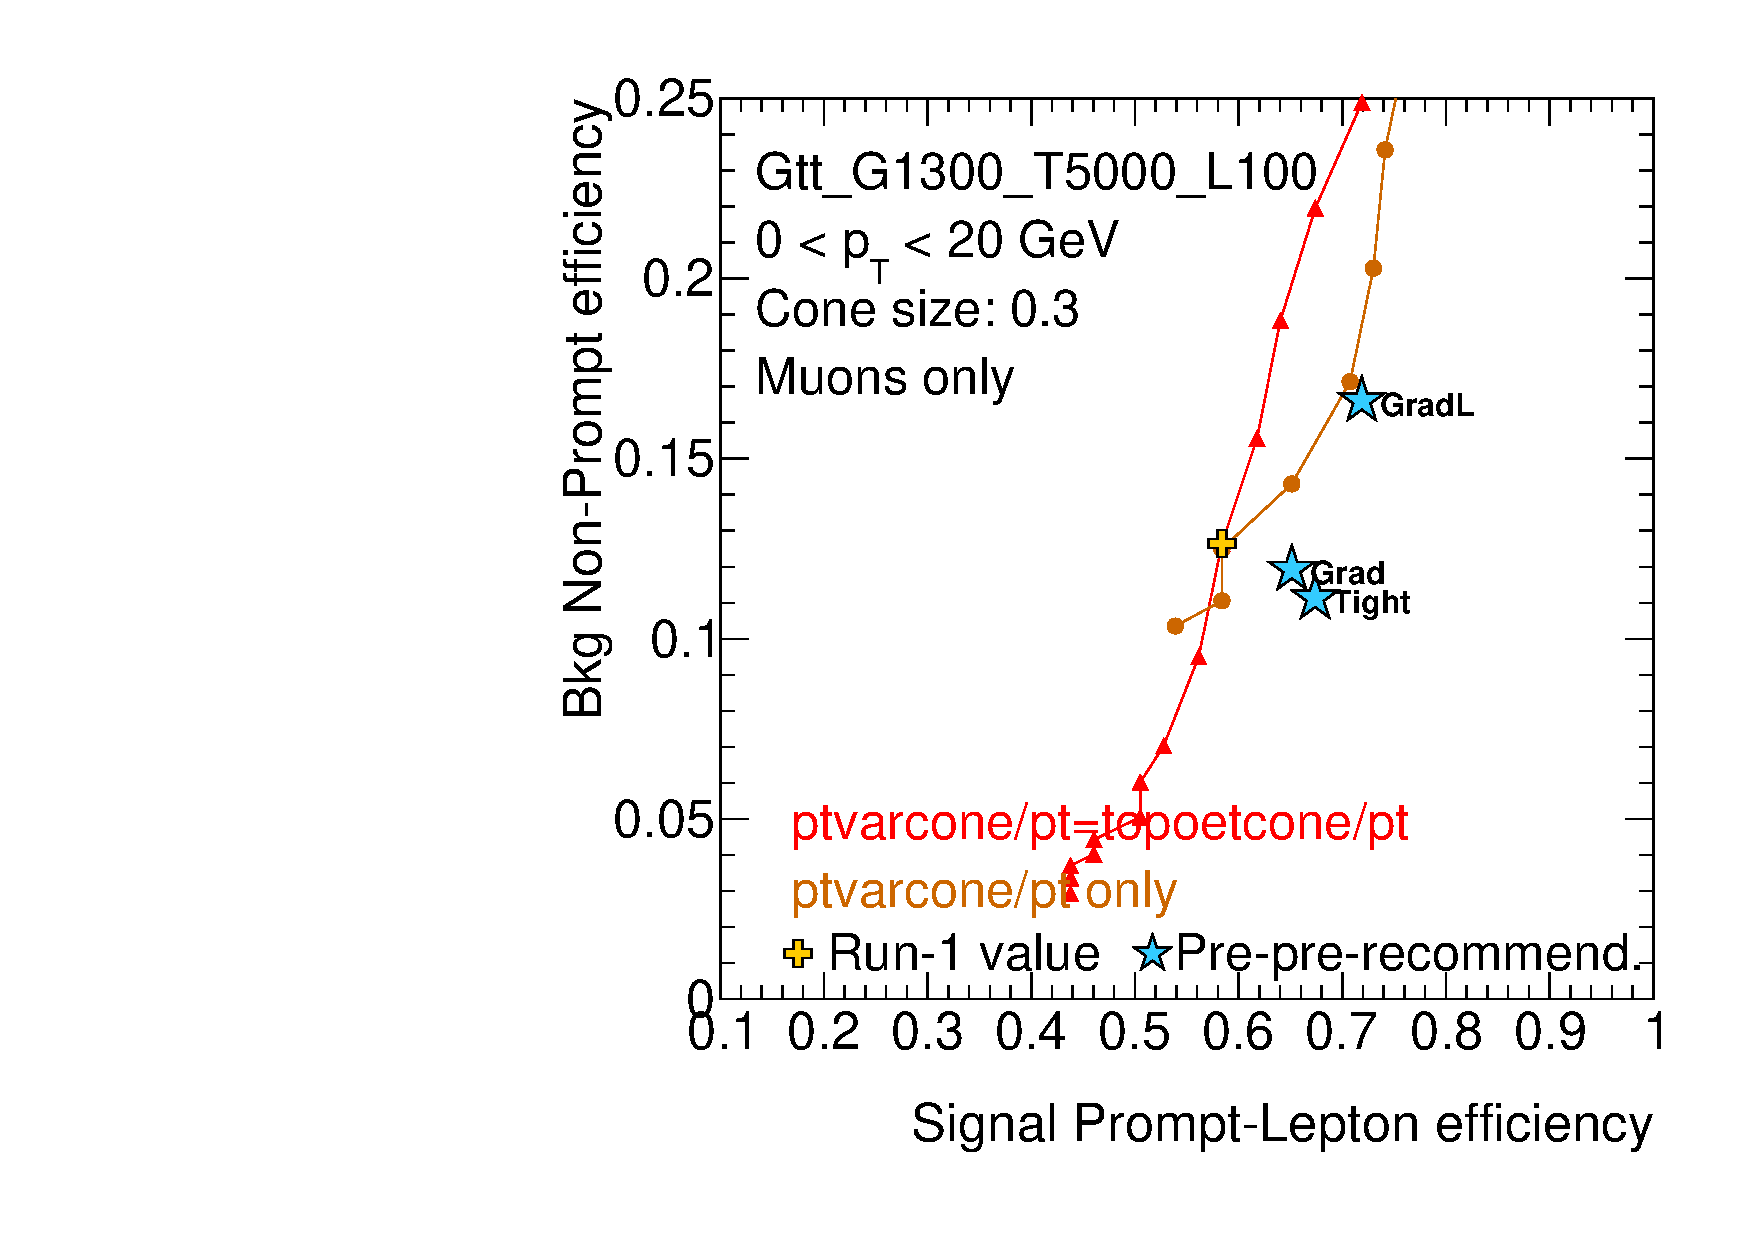
\includegraphics[width=0.4\textwidth]{ISOLATION/Gtt_G1300_T5000_L100_pt1-1_cone30_id13_pre_med.pdf}
%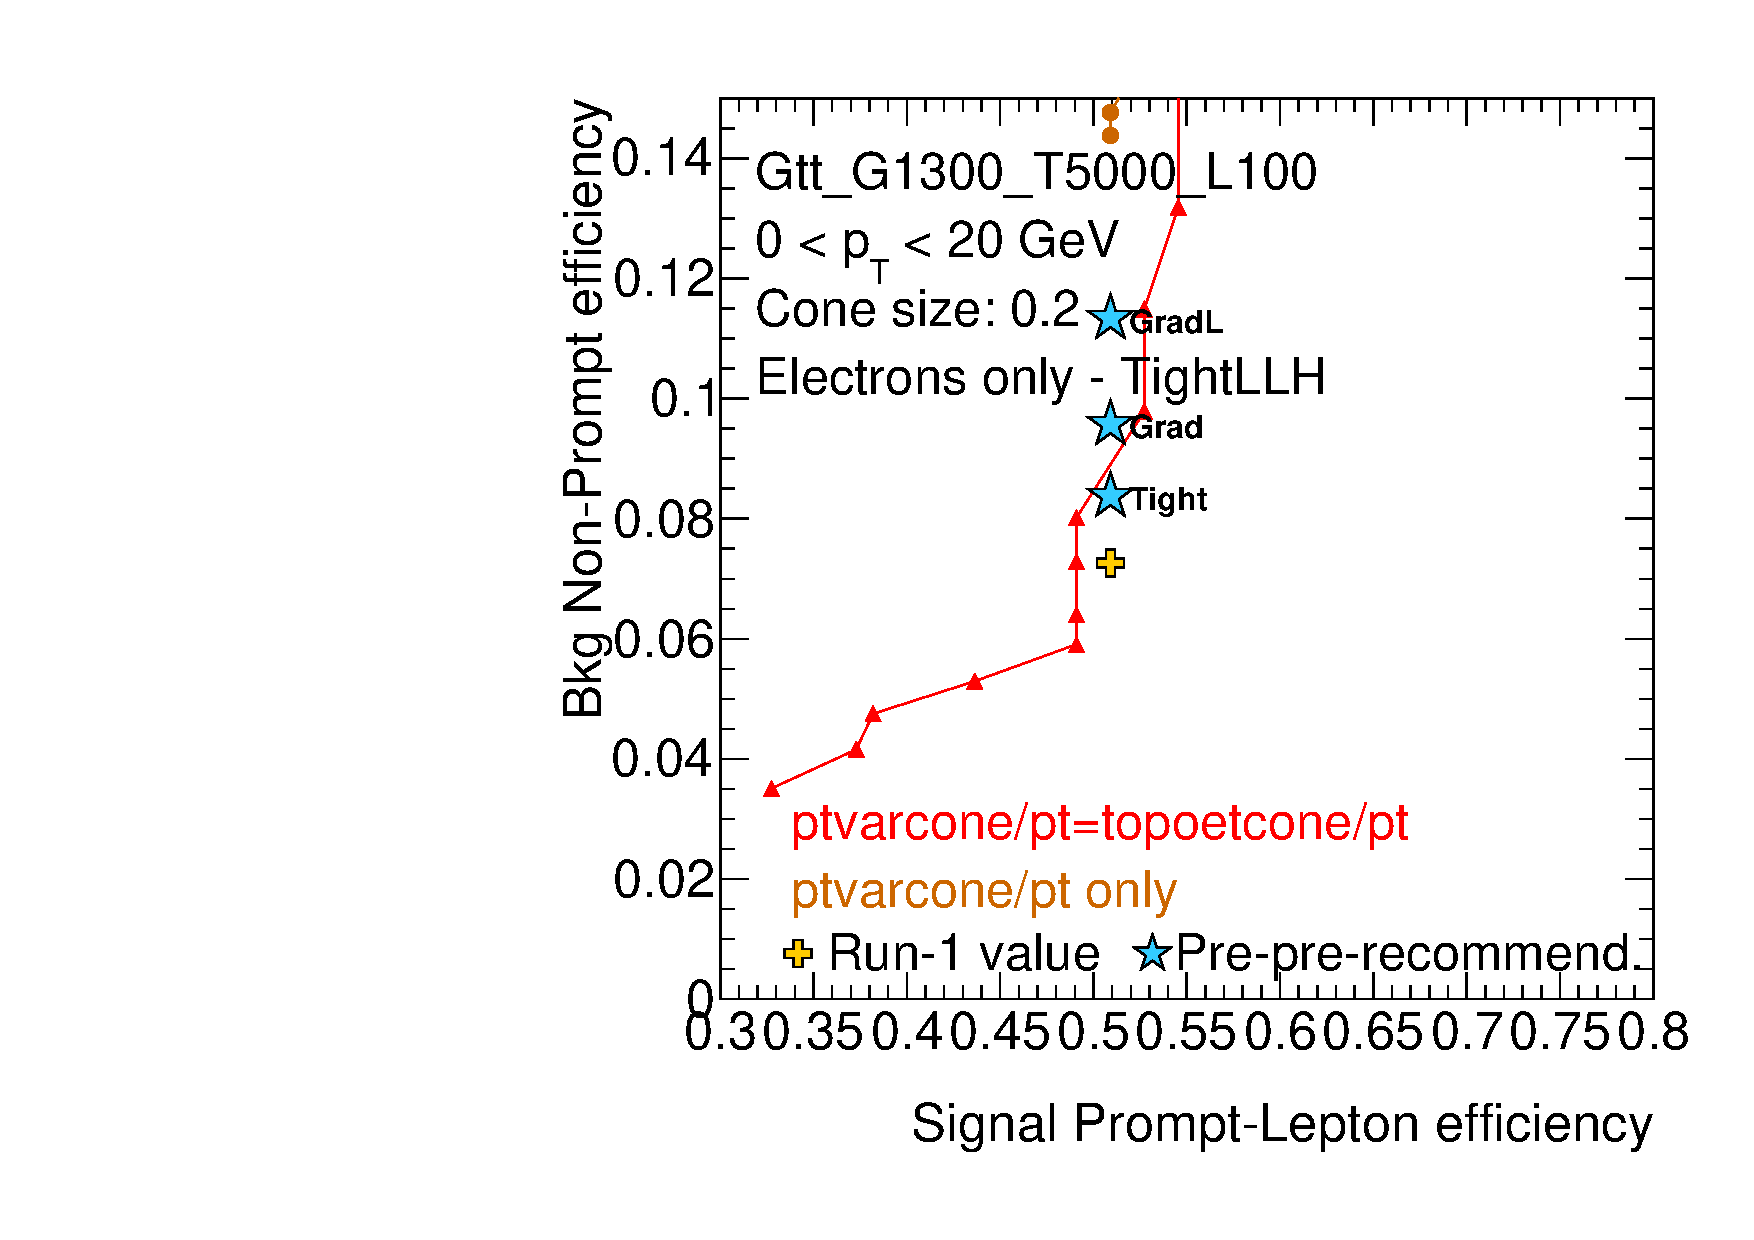
\includegraphics[width=0.4\textwidth]{ISOLATION/Gtt_G1300_T5000_L100_pt1-1_cone20_id11_pre.pdf}
%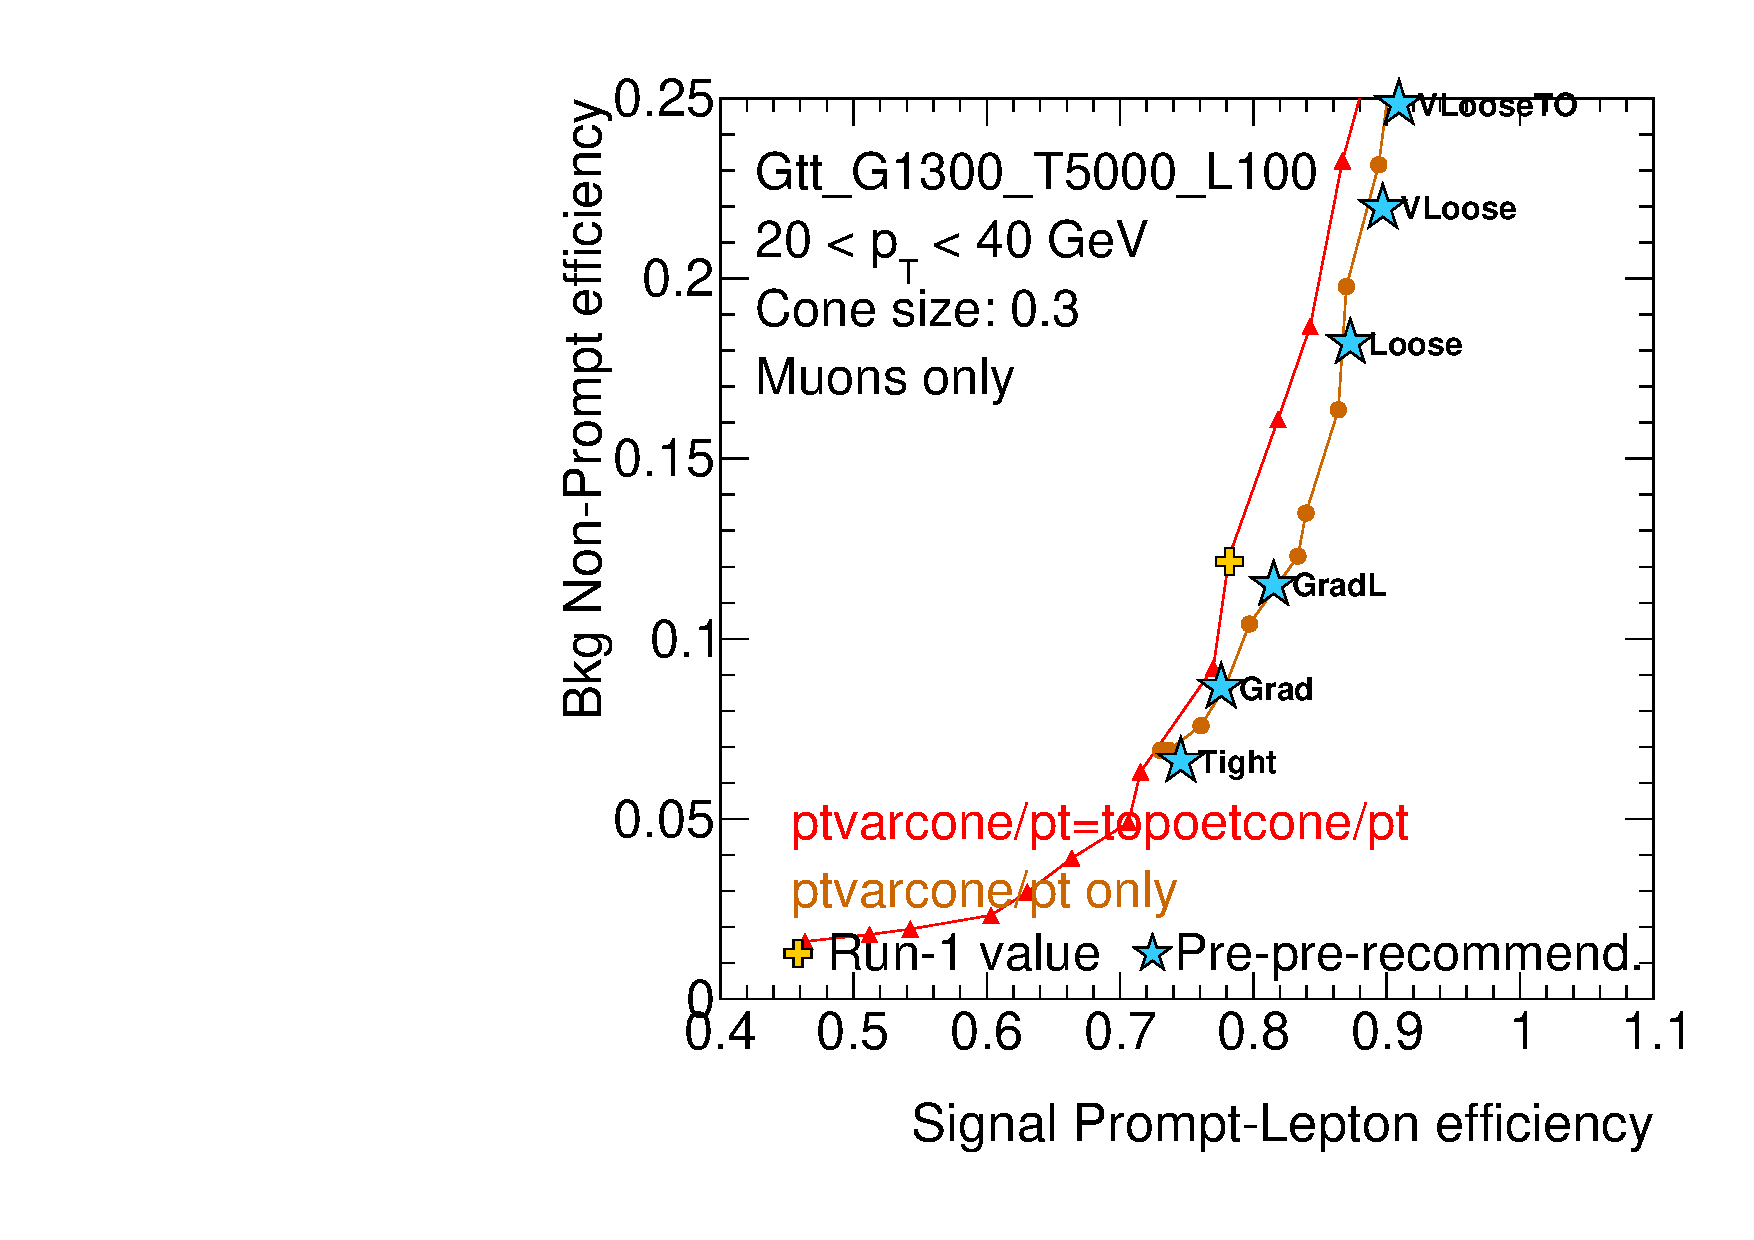
\includegraphics[width=0.4\textwidth]{ISOLATION/Gtt_G1300_T5000_L100_pt2-2_cone30_id13_pre_med.pdf}
%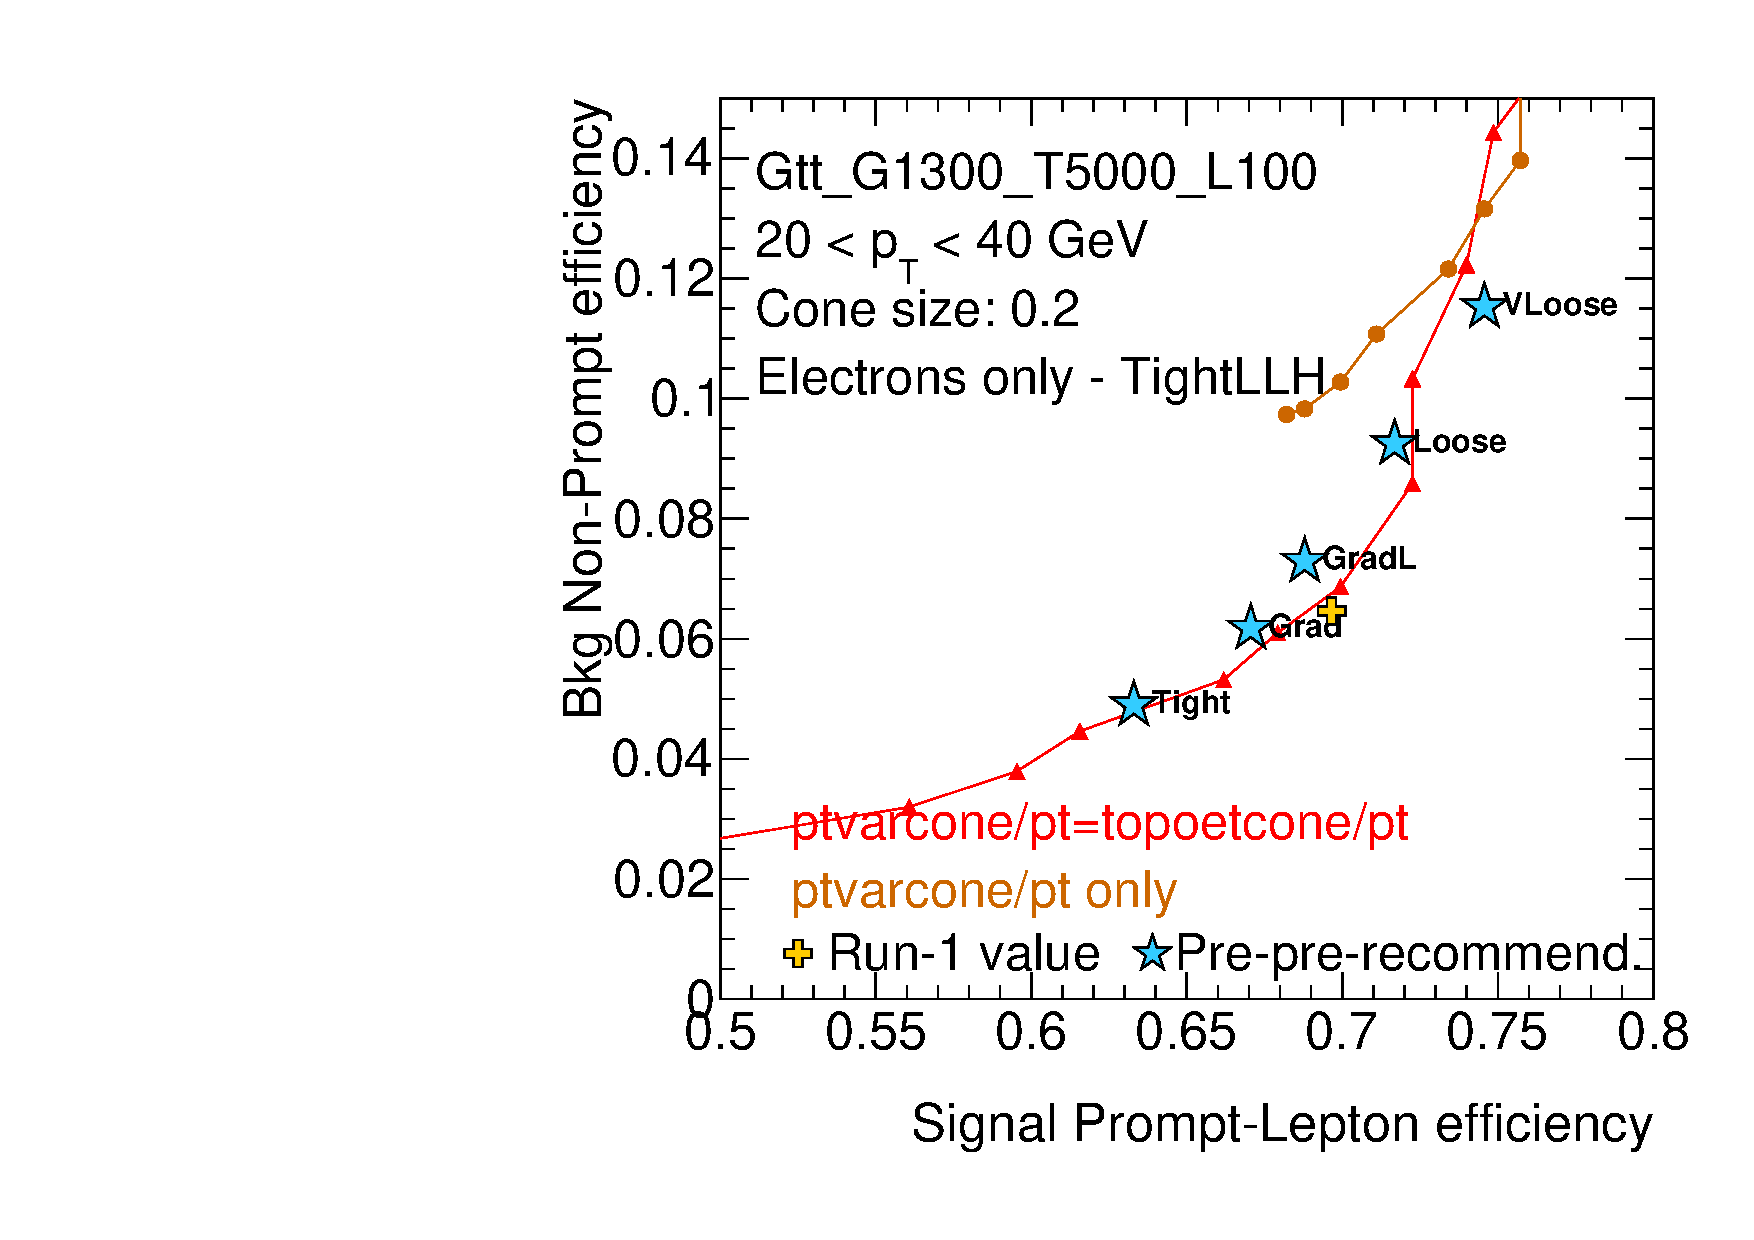
\includegraphics[width=0.4\textwidth]{ISOLATION/Gtt_G1300_T5000_L100_pt2-2_cone20_id11_pre.pdf}
%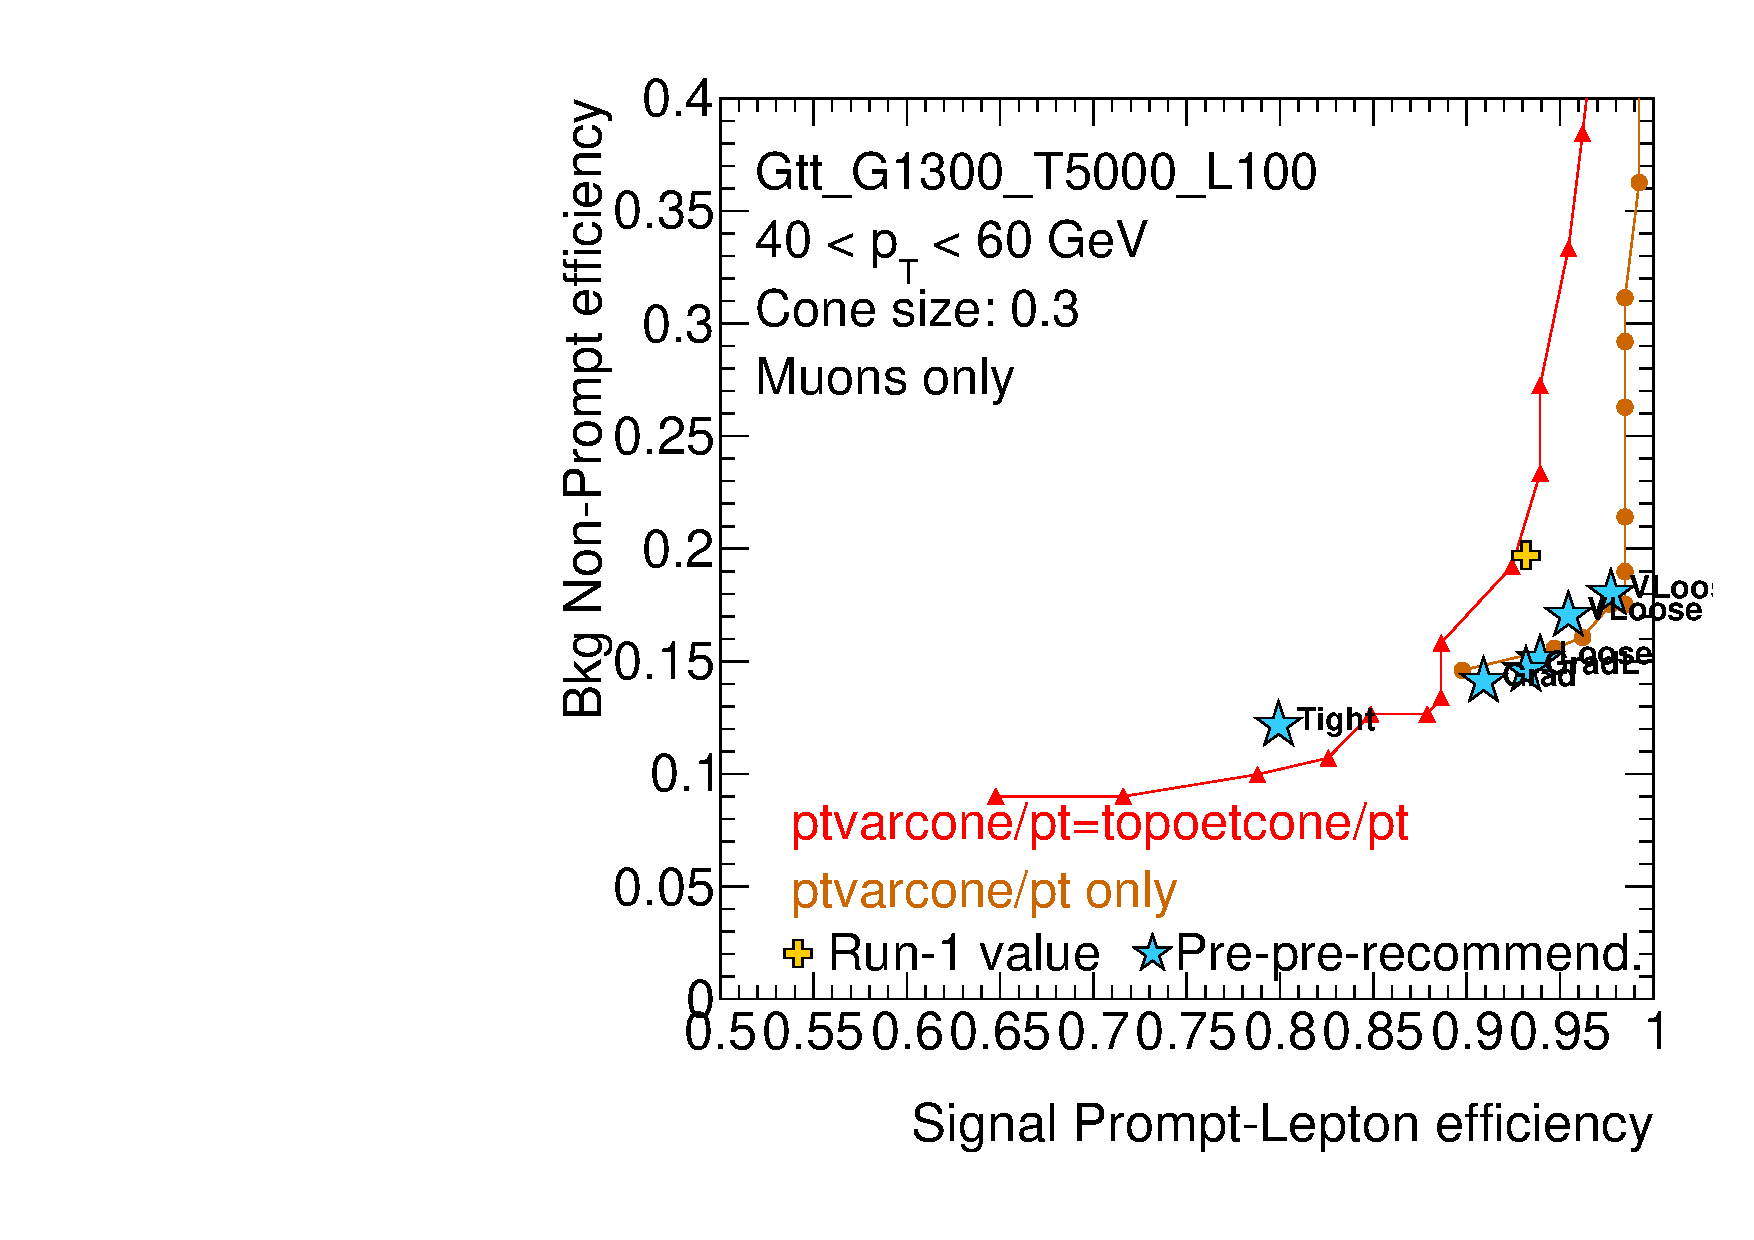
\includegraphics[width=0.4\textwidth]{ISOLATION/Gtt_G1300_T5000_L100_pt3-3_cone30_id13_pre_med.pdf}
%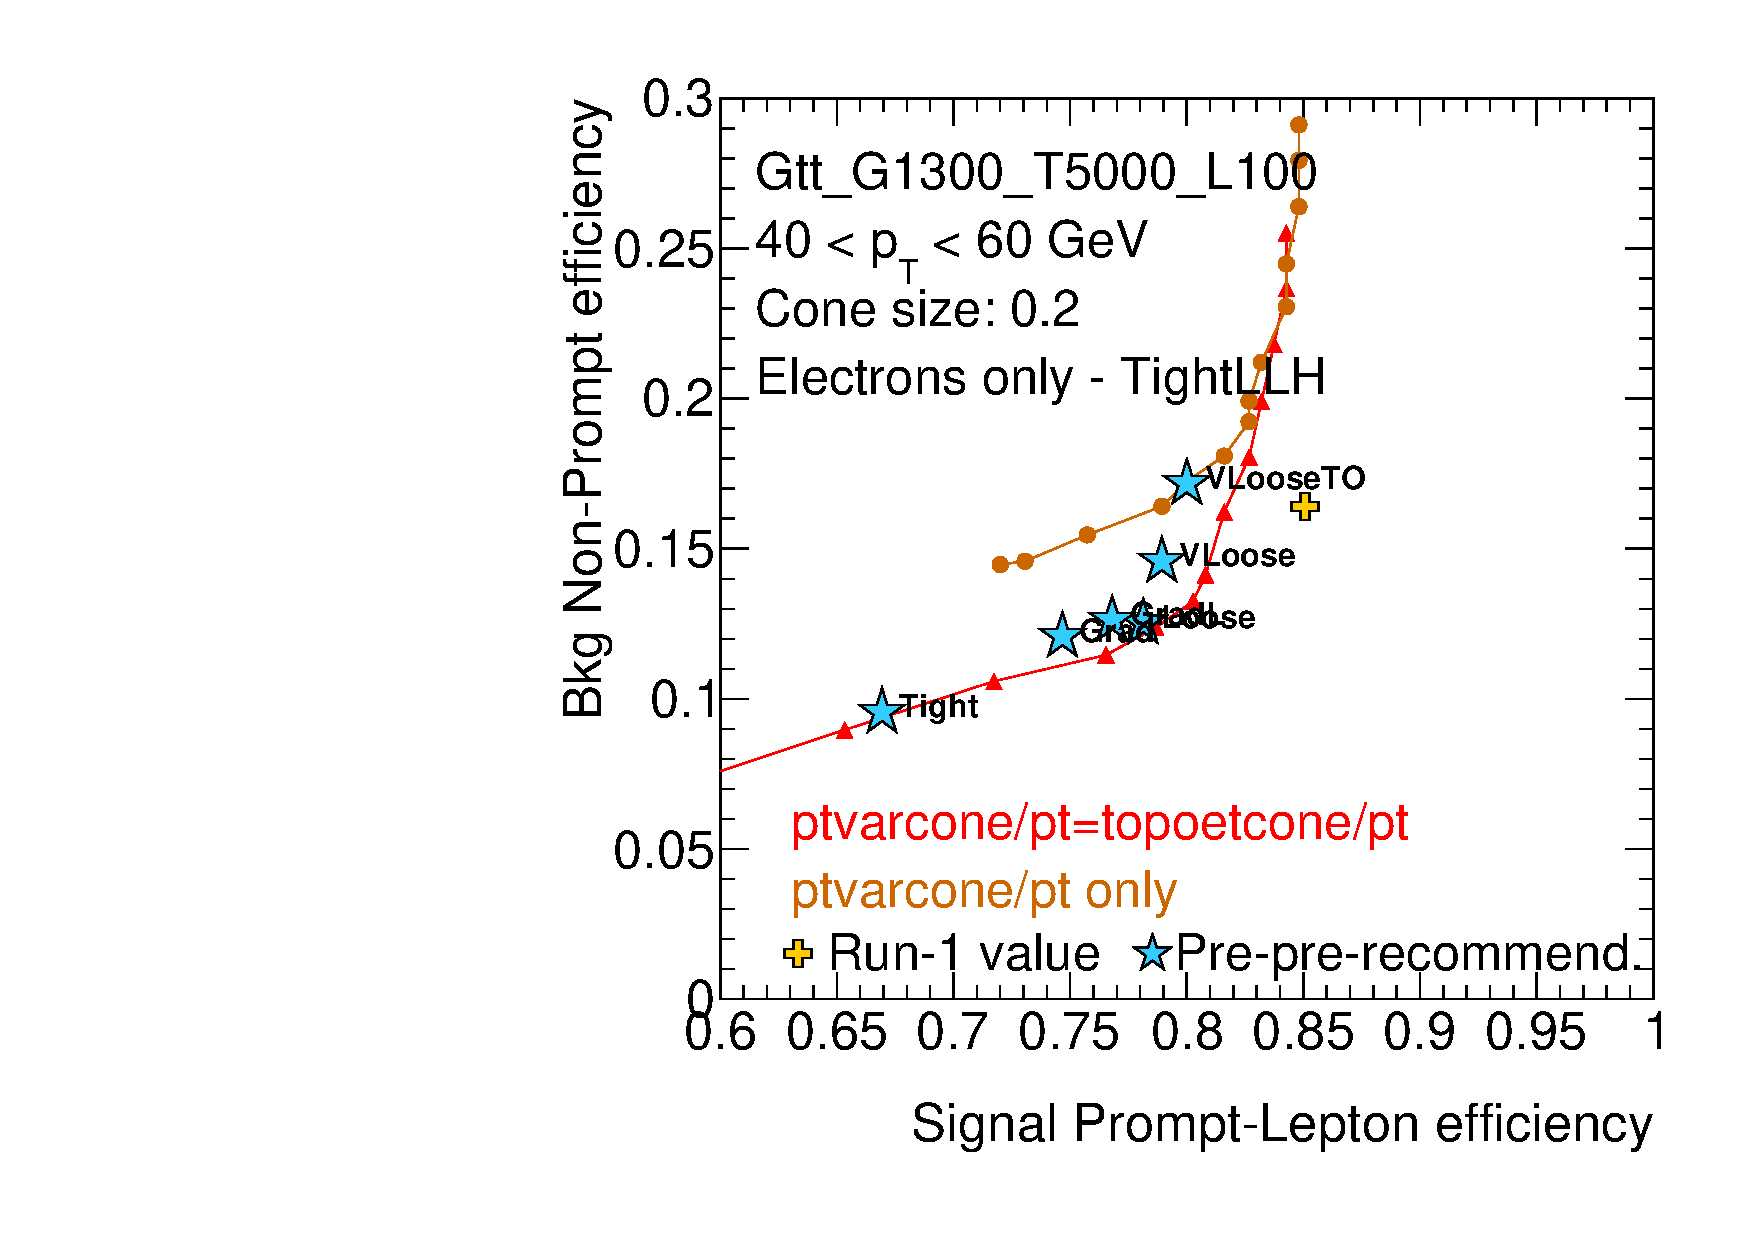
\includegraphics[width=0.4\textwidth]{ISOLATION/Gtt_G1300_T5000_L100_pt3-3_cone20_id11_pre.pdf}
%\end{center}
%\vspace{-0.2cm}
%\caption{Isolation efficiency for background non-prompt muons as a function of the isolation efficiency for prompt muons in signal events for muons (left) and electrons (right) in different $\pt$ bins in DC14 samples. Curves are shown for ptvarcone/\pt alone, ptvarcone/\pt combined with topoetcone/\pt and the isolation pre-pre-recommendations working points. In addition, the cross shows the value that would be obtained with settings equivalent to those used during Run-1.}
%\label{fig:isoDC14}
%\end{figure}

%Figure~\ref{fig:isoDC14} shows the isolation efficiency for non-prompt leptons in background samples and prompt leptons in a signal samples. Optimization studies considering both signal and background using the discovery significance as figure of merit showed that the {\tt GradientLoose} working point had a good performance for the signal regions in this analysis, and was therefore adopted as the isolaton definition for the lepton selection in the analysis.

On July 2015, the MC15 isolation pre-recommendations were released by the ATLAS isolation forum~\cite{IsoSel_twiki} which kept 
the definition of the {\tt GradientLoose} working point, as well as the isolation variables used to build it, unchanged. 
Figure~\ref{fig:isoMC15} shows the isolation efficiency for non-prompt leptons in background samples and prompt leptons in a signal sample, with a much higher fake muon efficiency compared to the Run-1 or DC14 studies (\cite{NoteDC14}). 
This was traced to be due to much looser cuts applied to the ptvarcone30/\pt inside the {\tt IsolationSelectionTool} 
for low-\pt muons, as detailed in Appendix~\ref{app:iso}.

\begin{figure}[phtb!]
\begin{center}
\includegraphics[page=2,width=0.4\textwidth]{ISOLATION/roc.pdf}
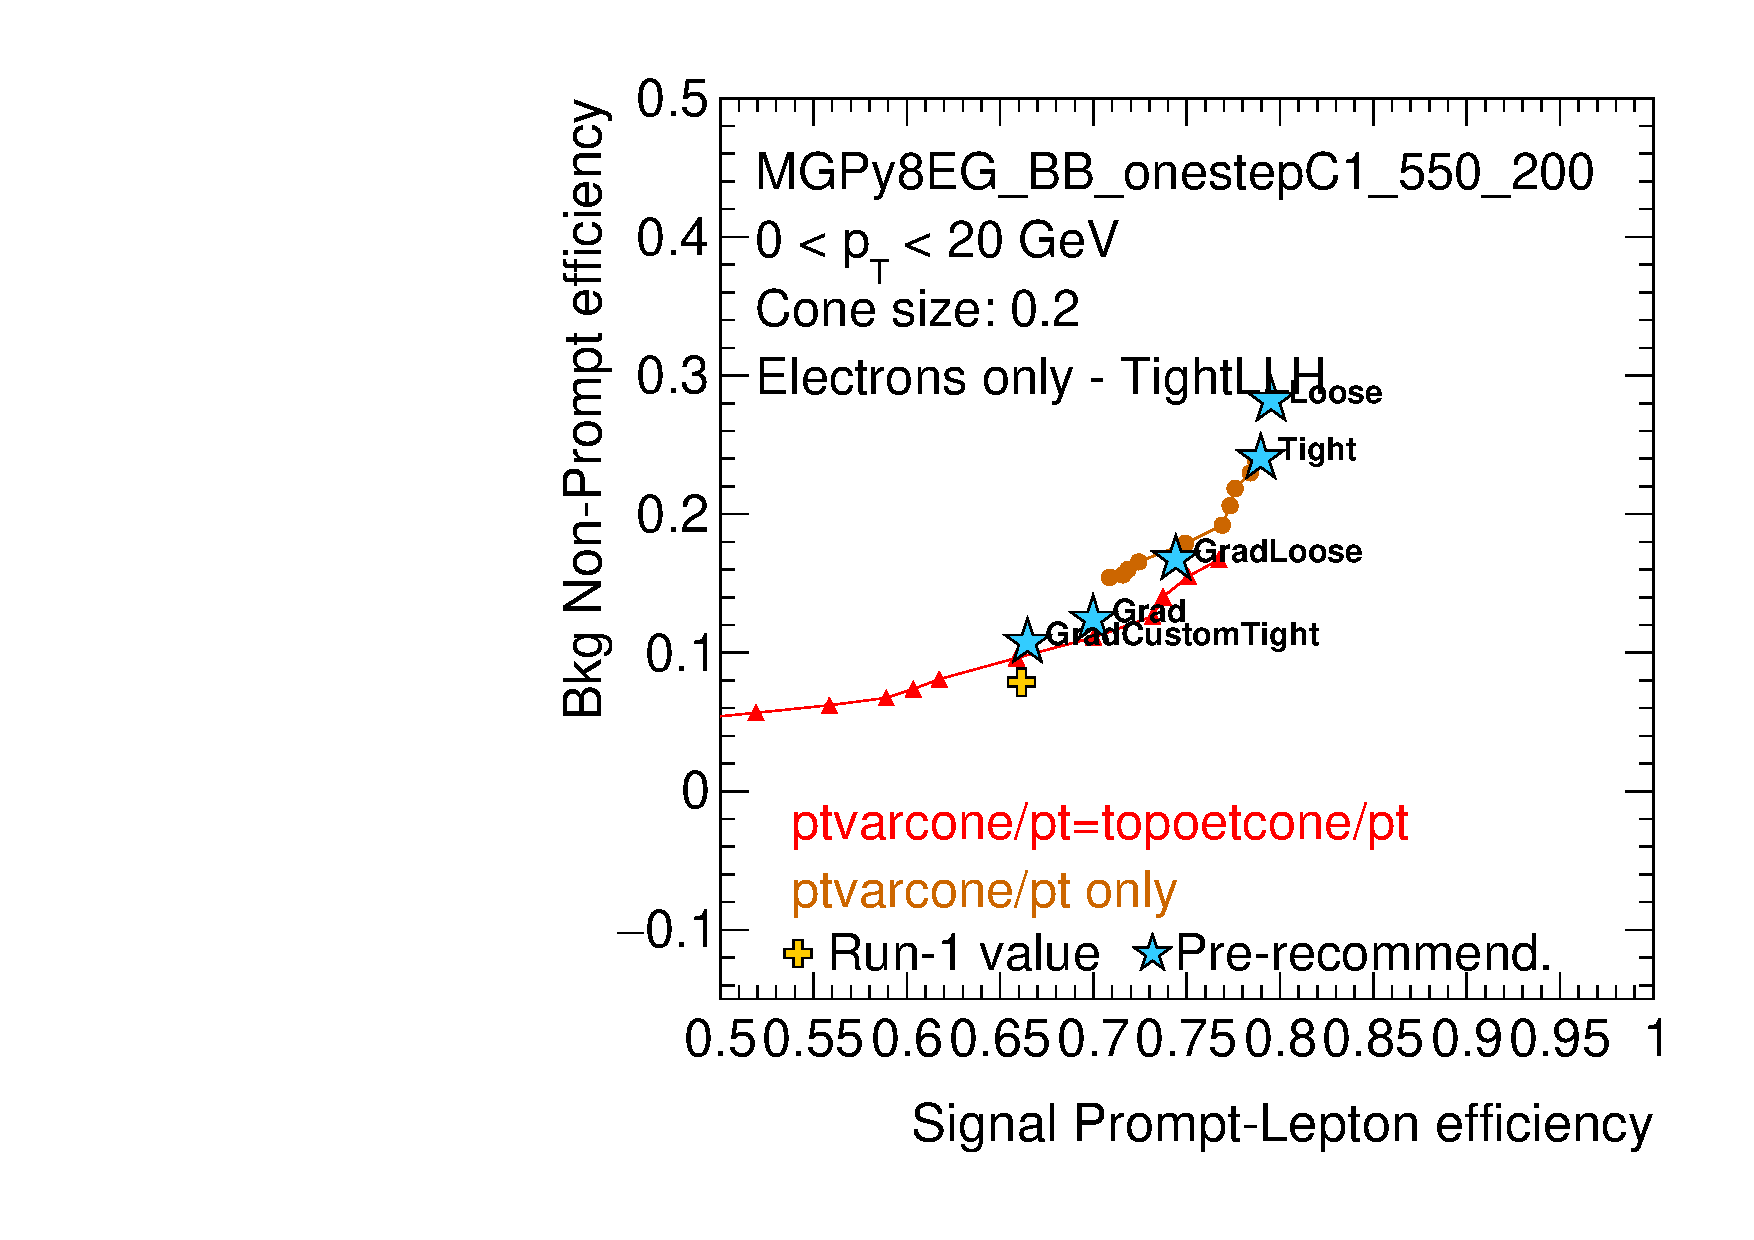
\includegraphics[page=1,width=0.4\textwidth]{ISOLATION/roc.pdf}
\includegraphics[page=4,width=0.4\textwidth]{ISOLATION/roc.pdf}
\includegraphics[page=3,width=0.4\textwidth]{ISOLATION/roc.pdf}
\includegraphics[page=6,width=0.4\textwidth]{ISOLATION/roc.pdf}
\includegraphics[page=5,width=0.4\textwidth]{ISOLATION/roc.pdf}
\end{center}
\vspace{-0.2cm}
\caption{Isolation efficiency for background non-prompt muons as a function of the isolation efficiency for prompt muons in signal events for muons (left) and electrons (right) in different $\pt$ bins in MC15 samples. Curves are shown for ptvarcone/\pt alone, ptvarcone/\pt combined with topoetcone/\pt and the isolation pre-recommendations working points. In addition, the cross shows the value that would be obtained with settings equivalent to those used during Run-1.}
\label{fig:isoMC15}
\end{figure}

Two additional custom isolation working points were defined with  the same variable efficiency approach used for {\tt Gradient} and {\tt GradientLoose} but with much tighter settings. The isolation efficiency for these two custom working points is the following:
\begin{itemize}
\item {\tt GradientCustom}: (0.1713$\times$\pt[GeV]+88.71)\%
\item {\tt GradientCustomTight}: (0.2283$\times$\pt[GeV]+85.28)\%
\end{itemize}
The prompt and non-prompt lepton efficiency for these working points is also shown in Figure~\ref{fig:isoMC15}, and they are able to recover the rejection against non-prompt leptons to levels comparable to those in Run-1. A scan over the isolation working points in terms of discovery significance for a couple of signal models is shown in Figure~\ref{fig:IsoScan}. The significance is computed after a selection of two same-sign leptons, 4 jets with $\pt >50$~GeV and $\met>100$ GeV assuming 3~fb$^{-1}$ of integrated luminosity and a 30\% background uncertainty. As shown, {\tt GradientLoose} is not optimal, with significances $\sim$10\% lower than the most performing configuration, and the customly defined working points are strongly preferred, with the simple cuts on the isolation variables used in DC14 (``eVTmT'', also referred to as ``EL0p06'' and ``MU0p06'') providing very competitive results.

\begin{figure}[phtb!]
\begin{center}
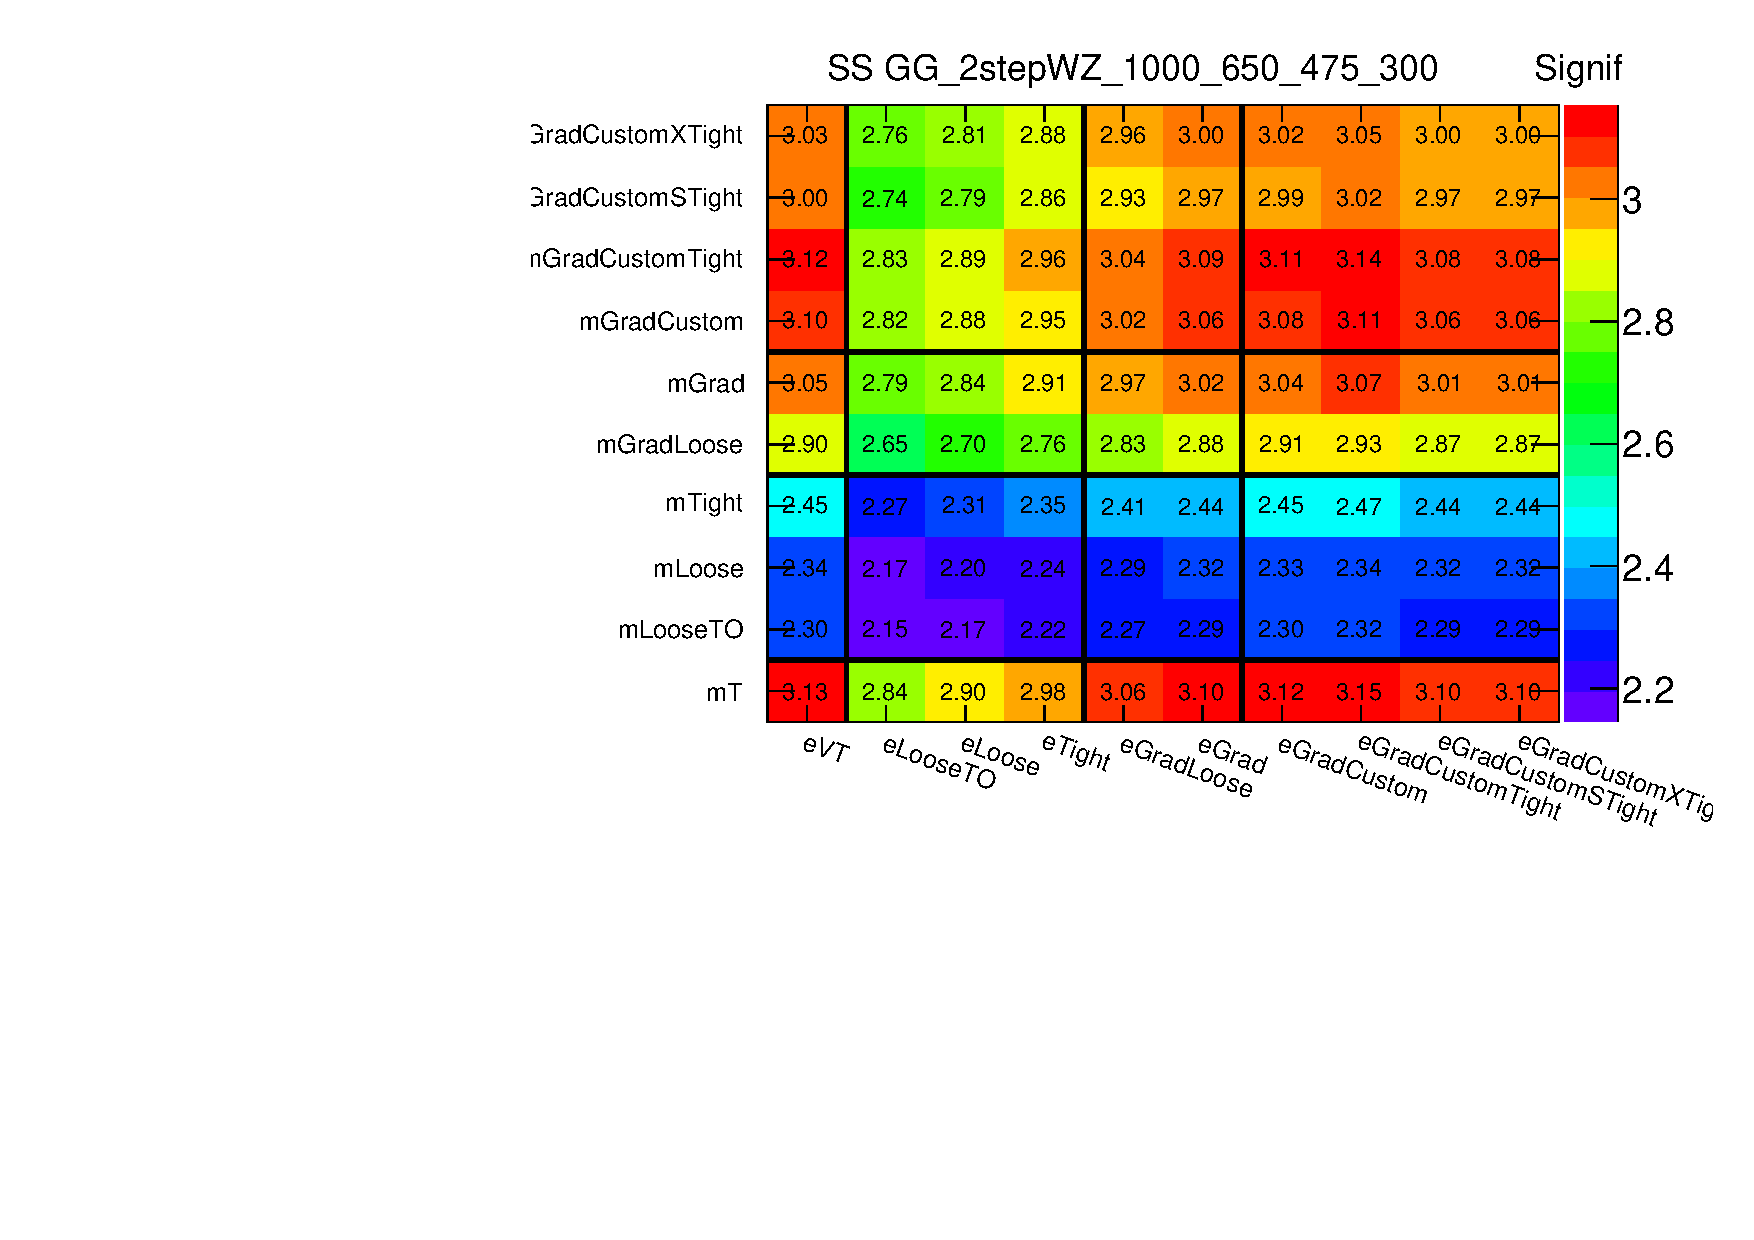
\includegraphics[width=0.6\textwidth]{ISOLATION/SS_Signif_SMGG2WWZZ_1000_530_60.pdf}
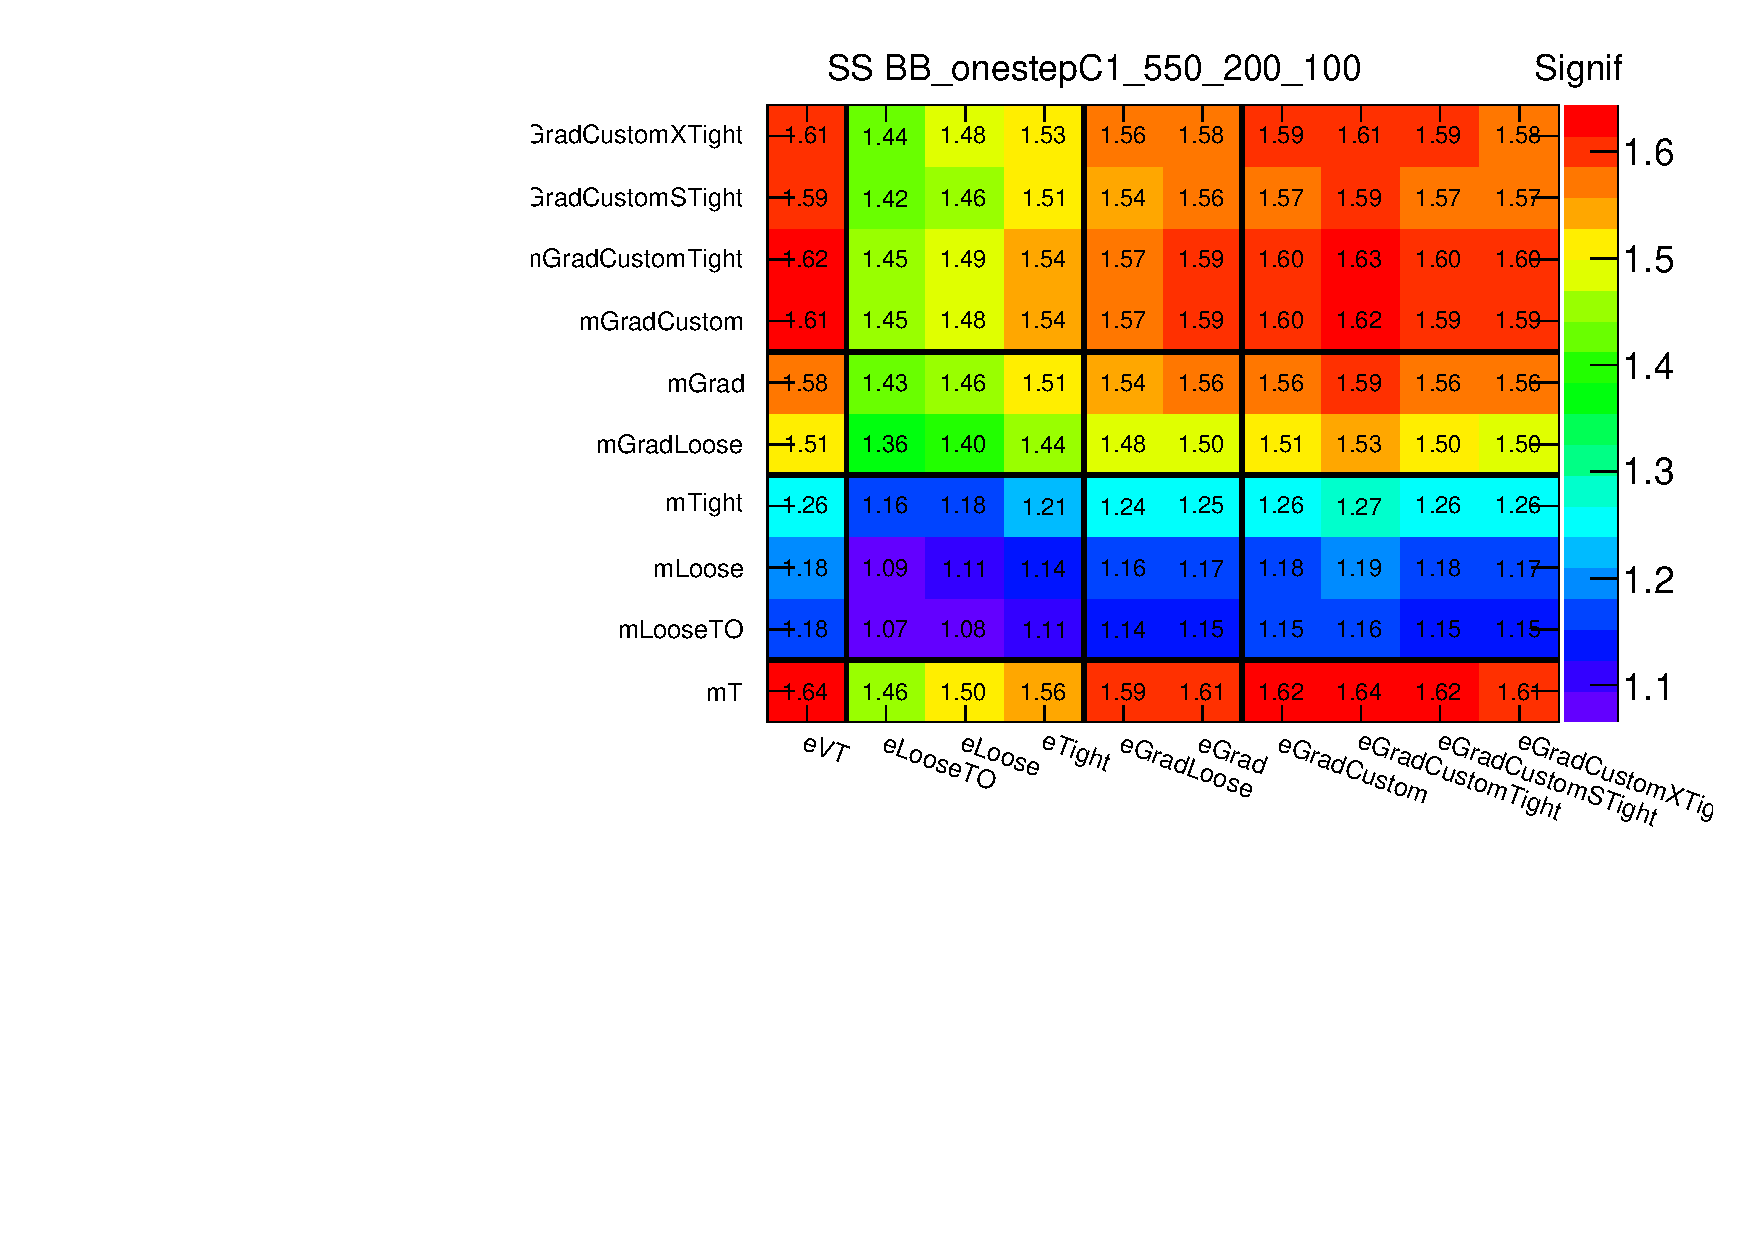
\includegraphics[width=0.6\textwidth]{ISOLATION/SS_Signif_BB_onestepC1_550_200_100.pdf}
\end{center}
\vspace{-0.2cm}
\caption{Discovery significance values for different isolation requirements on electrons (x-axis) and muons (y-axis) for 2~\ifb. }
\label{fig:IsoScan}
\end{figure}

The isolation working points proposed from this analysis were accepted by the ATLAS Isolation forum and implemented as officially supported working points in the {\tt IsolationSelectionTool}. In the studies contained in this note, ``FixedCutTight'' and ``FixedCutTightTrackOnly'' are used unless otherwise stated.
